%!TEX root = main.tex
\label{cap:sec2}
% What relevant differences in security performance does your metric reveal
%ToDo : cite owr first article
In this section we analize the output of the metrics proposed in~\cite{owr_article}. Based on this output we compare the performance of the distinct network owners. We detail how the security performance can me compared using applying the metrics to a subset of the the problem owners i.e. ISPs in China.
% consider costumer, address space and services

\subsection{BN propagation}
This metric can be used to measure the evolution of the botnet in side a network. Since each ISP know the number of clients this metric can be normalized using this value. If an external party would like to compute and compare its perfromance using this metric, the normalization can be performed using the number of IP available addresses.

% Overal growth (per network ?)
% Total cost ?
\subsection{Network infection radio}


\begin{figure}[h]
    % \caption{}
    % \label{fig:agg_grow}
    \centering
    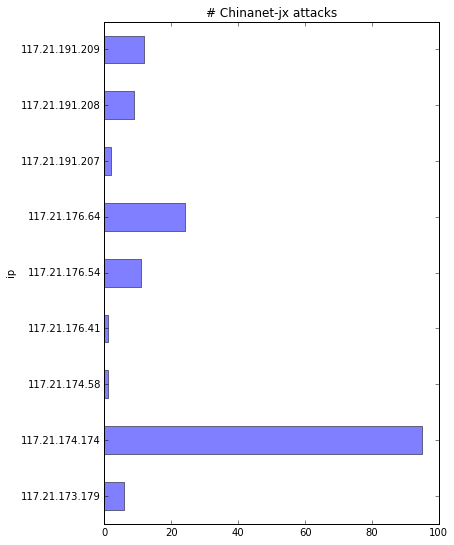
\includegraphics[width=\linewidth]{cn-jx}
\end{figure}


\begin{figure}[h]
    % \caption{}
    % \label{fig:agg_grow}
    \centering
    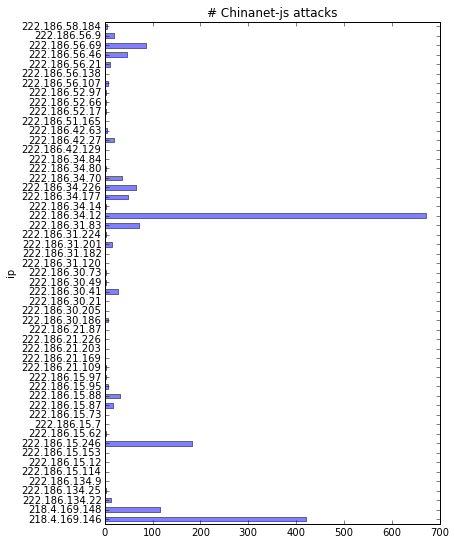
\includegraphics[width=\linewidth]{cn-js}
\end{figure}
% % Infection ratio between net owners
\subsection{BN geographical and digital location}
